\documentclass{article}
\usepackage[a4paper,margin=3cm,footskip=.5cm]{geometry}
\usepackage{amsmath,amssymb,amsthm,amsfonts,mdframed,kotex}
%\newcounter{problem}
\newcommand{\bp}[1]
{\begin{mdframed}
[frametitle={#1},skipabove=10pt,skipbelow=10pt]}
\newcommand{\ep}{\end{mdframed}}
\newcommand{\parall}{\mathbin{\!/\mkern-5mu/\!}}
\mdfsetup{nobreak=true}

\title{미리-04:쎈수학 2-2}
\date{\today}
\author{}

\begin{document}
\maketitle
\newpage

\bp{0686}
\(AD=5\), \(BC=10\)이고 사다리꼴 \(ABCD\)의 넓이를 선분 \(AE\)가 이등분할 때, \(EC\)의 길이를 구하여라.
\par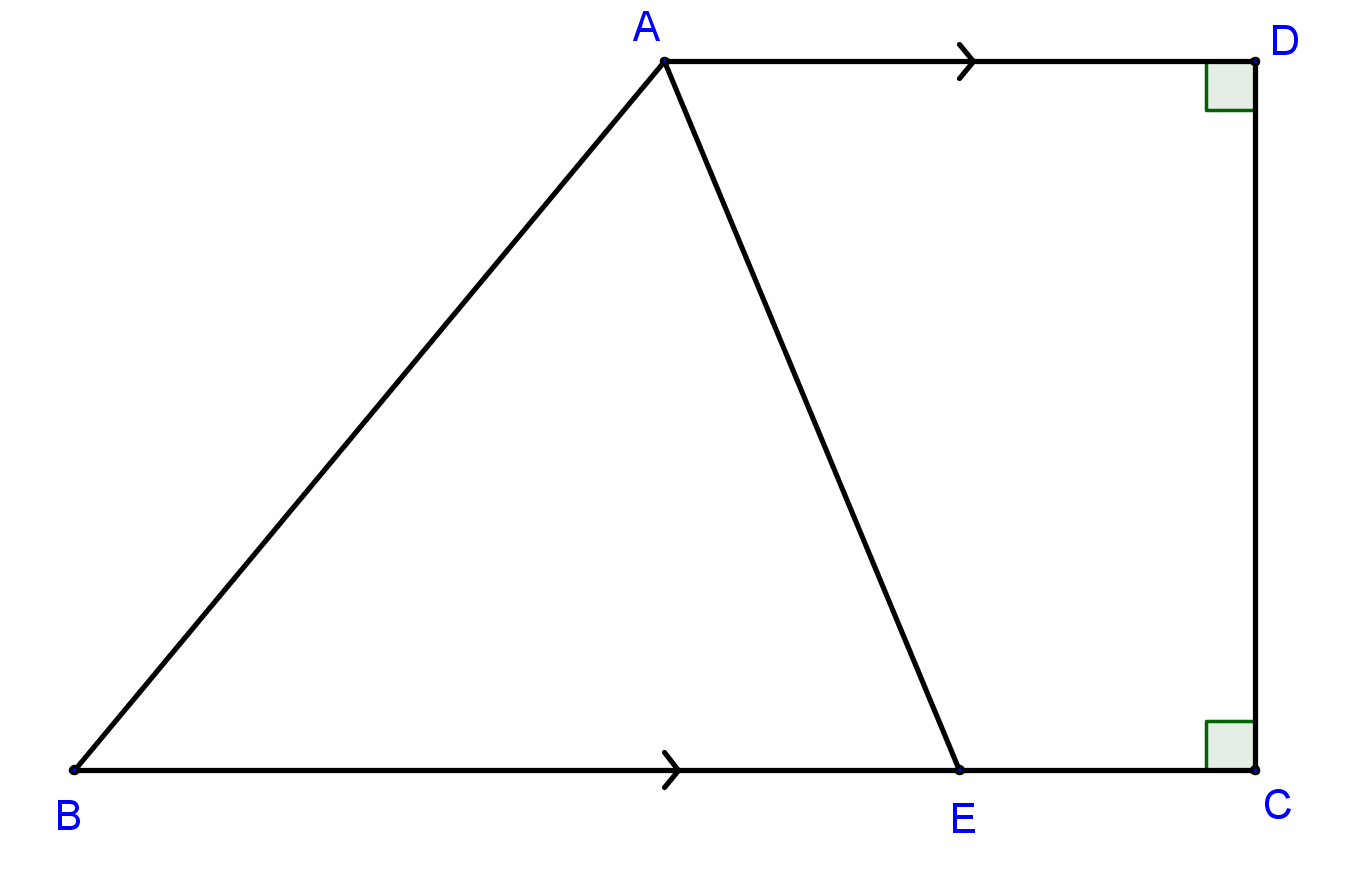
\includegraphics[width=0.5\textwidth]{SSEN_0686}
\ep

\bp{0700}
한 변의 길이가 \(13\)인 마름모 \(ABCD\)의 두 대각선의 길이가 각각 \(AC=10\), \(BD=24\)이다.
마름모 안의 한 점 \(P\)에서 네 변에 내린 수선의 길이를 각각 \(l_1\), \(l_2\), \(l_3\), \(l_4\)라고 할 때, \(l_1+l_2+l_3+l_4\)의 값을 구하시오.
\par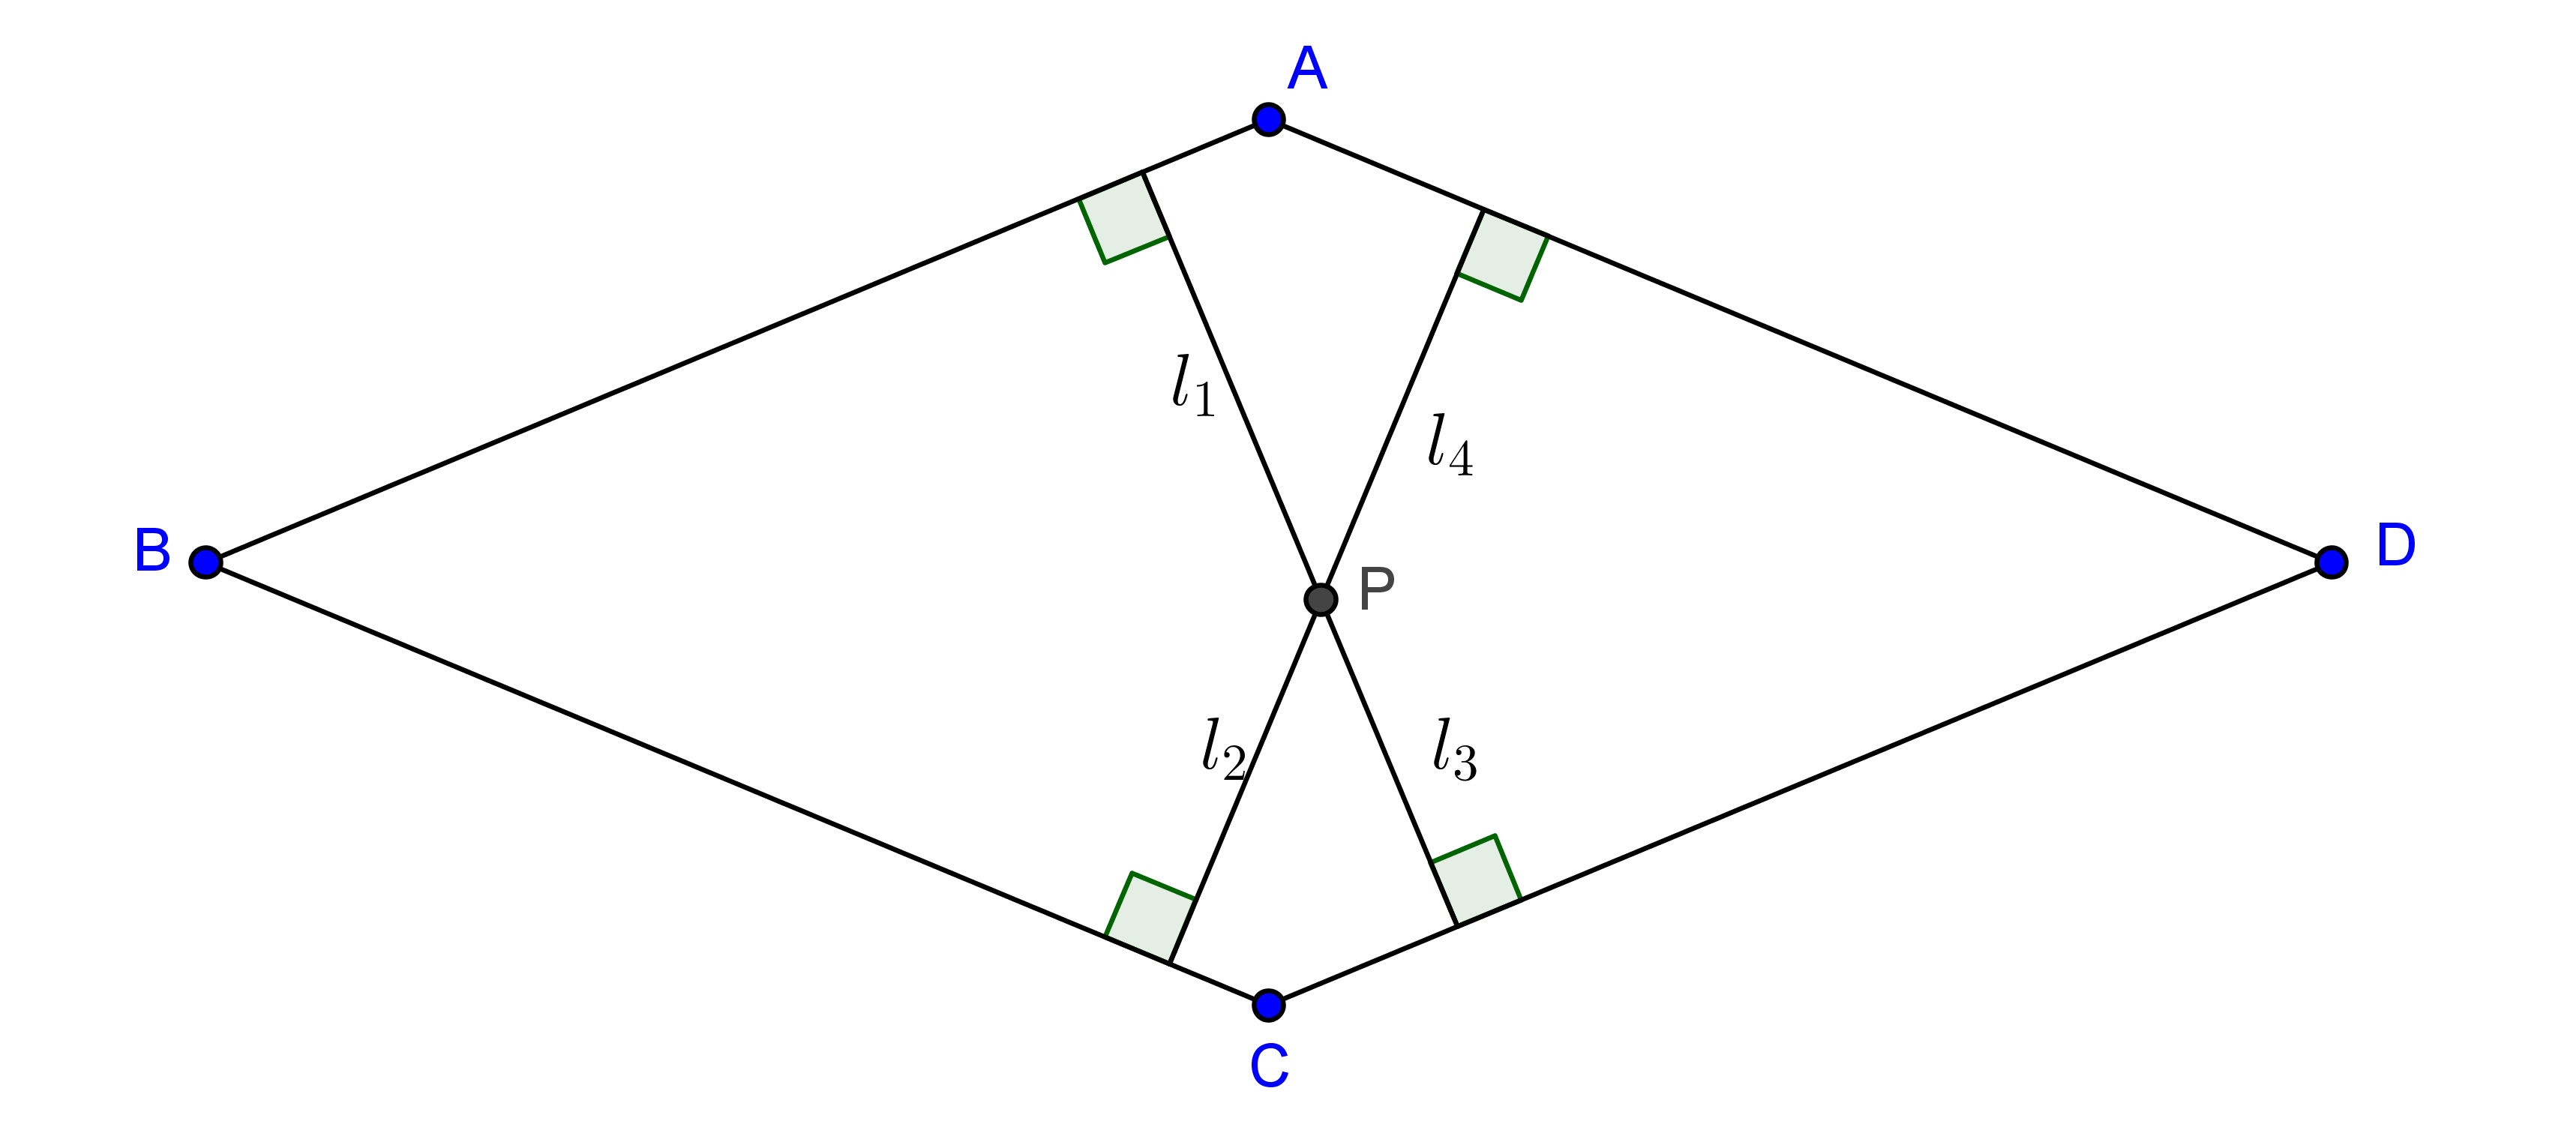
\includegraphics[width=0.5\textwidth]{SSEN_0700}
\ep

\bp{721}
\(AD\parall CD\)인 사다리꼴 \(ABCD\)모양의 땅이 \(PQ\)와 \(QR\)로 이루어진 경계선에 의해 두 부분으로 나누어져 있다.
두 땅의 넓이가 모두 변하지 않도록 하는 새로운 경계선 \(PS\)를 만들려고 할 때, \(S\)의 위치를 정하는 방법에 대해 서술하여라(단 \(S\)는 \(BC\)위의 점이다.).
\par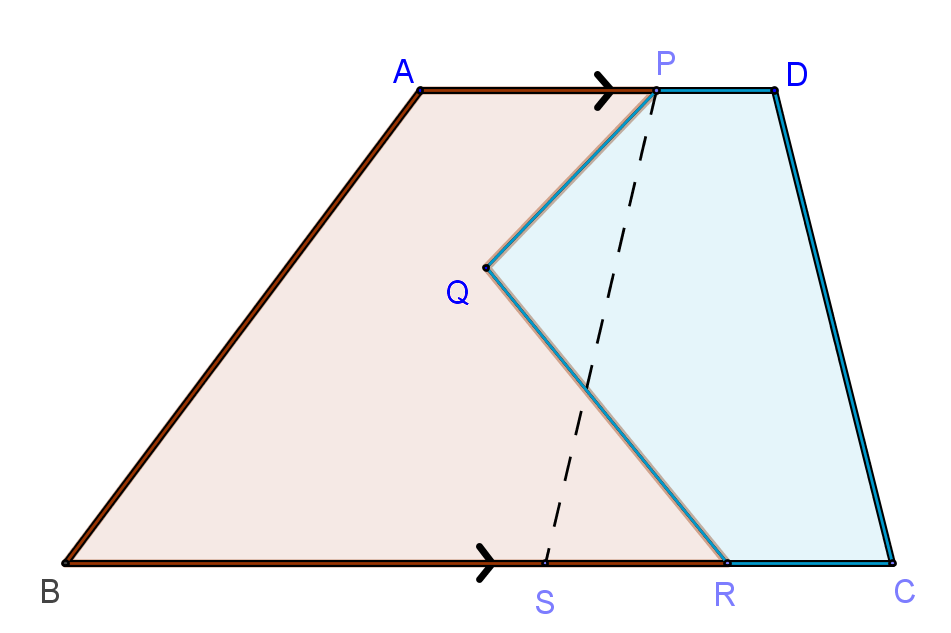
\includegraphics[width=0.5\textwidth]{SSEN_0721}
\ep

\bp{722}
\(AD:BC=2:3\)인 사다리꼴 \(ABCD\) 내부의 점 \(P\)에 대해 \(\triangle PAD=\triangle PBC\)이다.
\(\square ABCD=S\)라고 할 때, 색칠한 부분의 넓이를 \(S\)로 나타내어라.
\par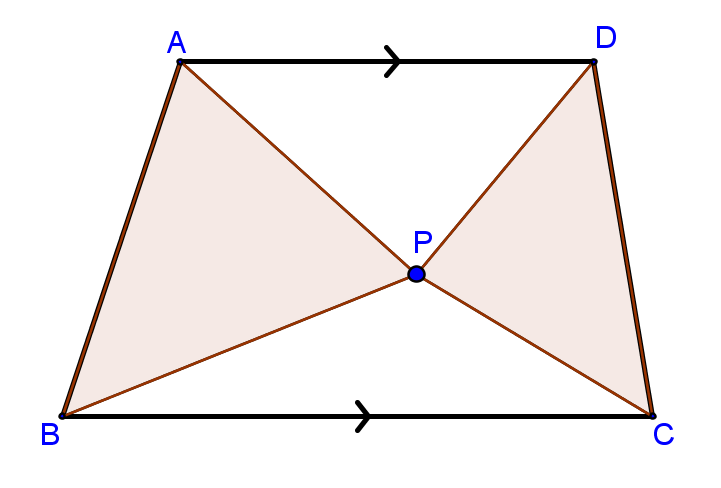
\includegraphics[width=0.5\textwidth]{SSEN_0722}
\ep

\bp{812}
다음과 같이 \(AD=20\)인 직사각형 \(ABCD\)가 있다.
서로 평행한 직선 \(l\), \(m\), \(n\), \(k\)가 \(BD\)를 5등분하고, \(l\)은 \(A\)를 지나며 \(k\)는 \(C\)를 지난다.
\(l\perp BD\)일 때, \(\square ABCD\)의 넓이는?
\par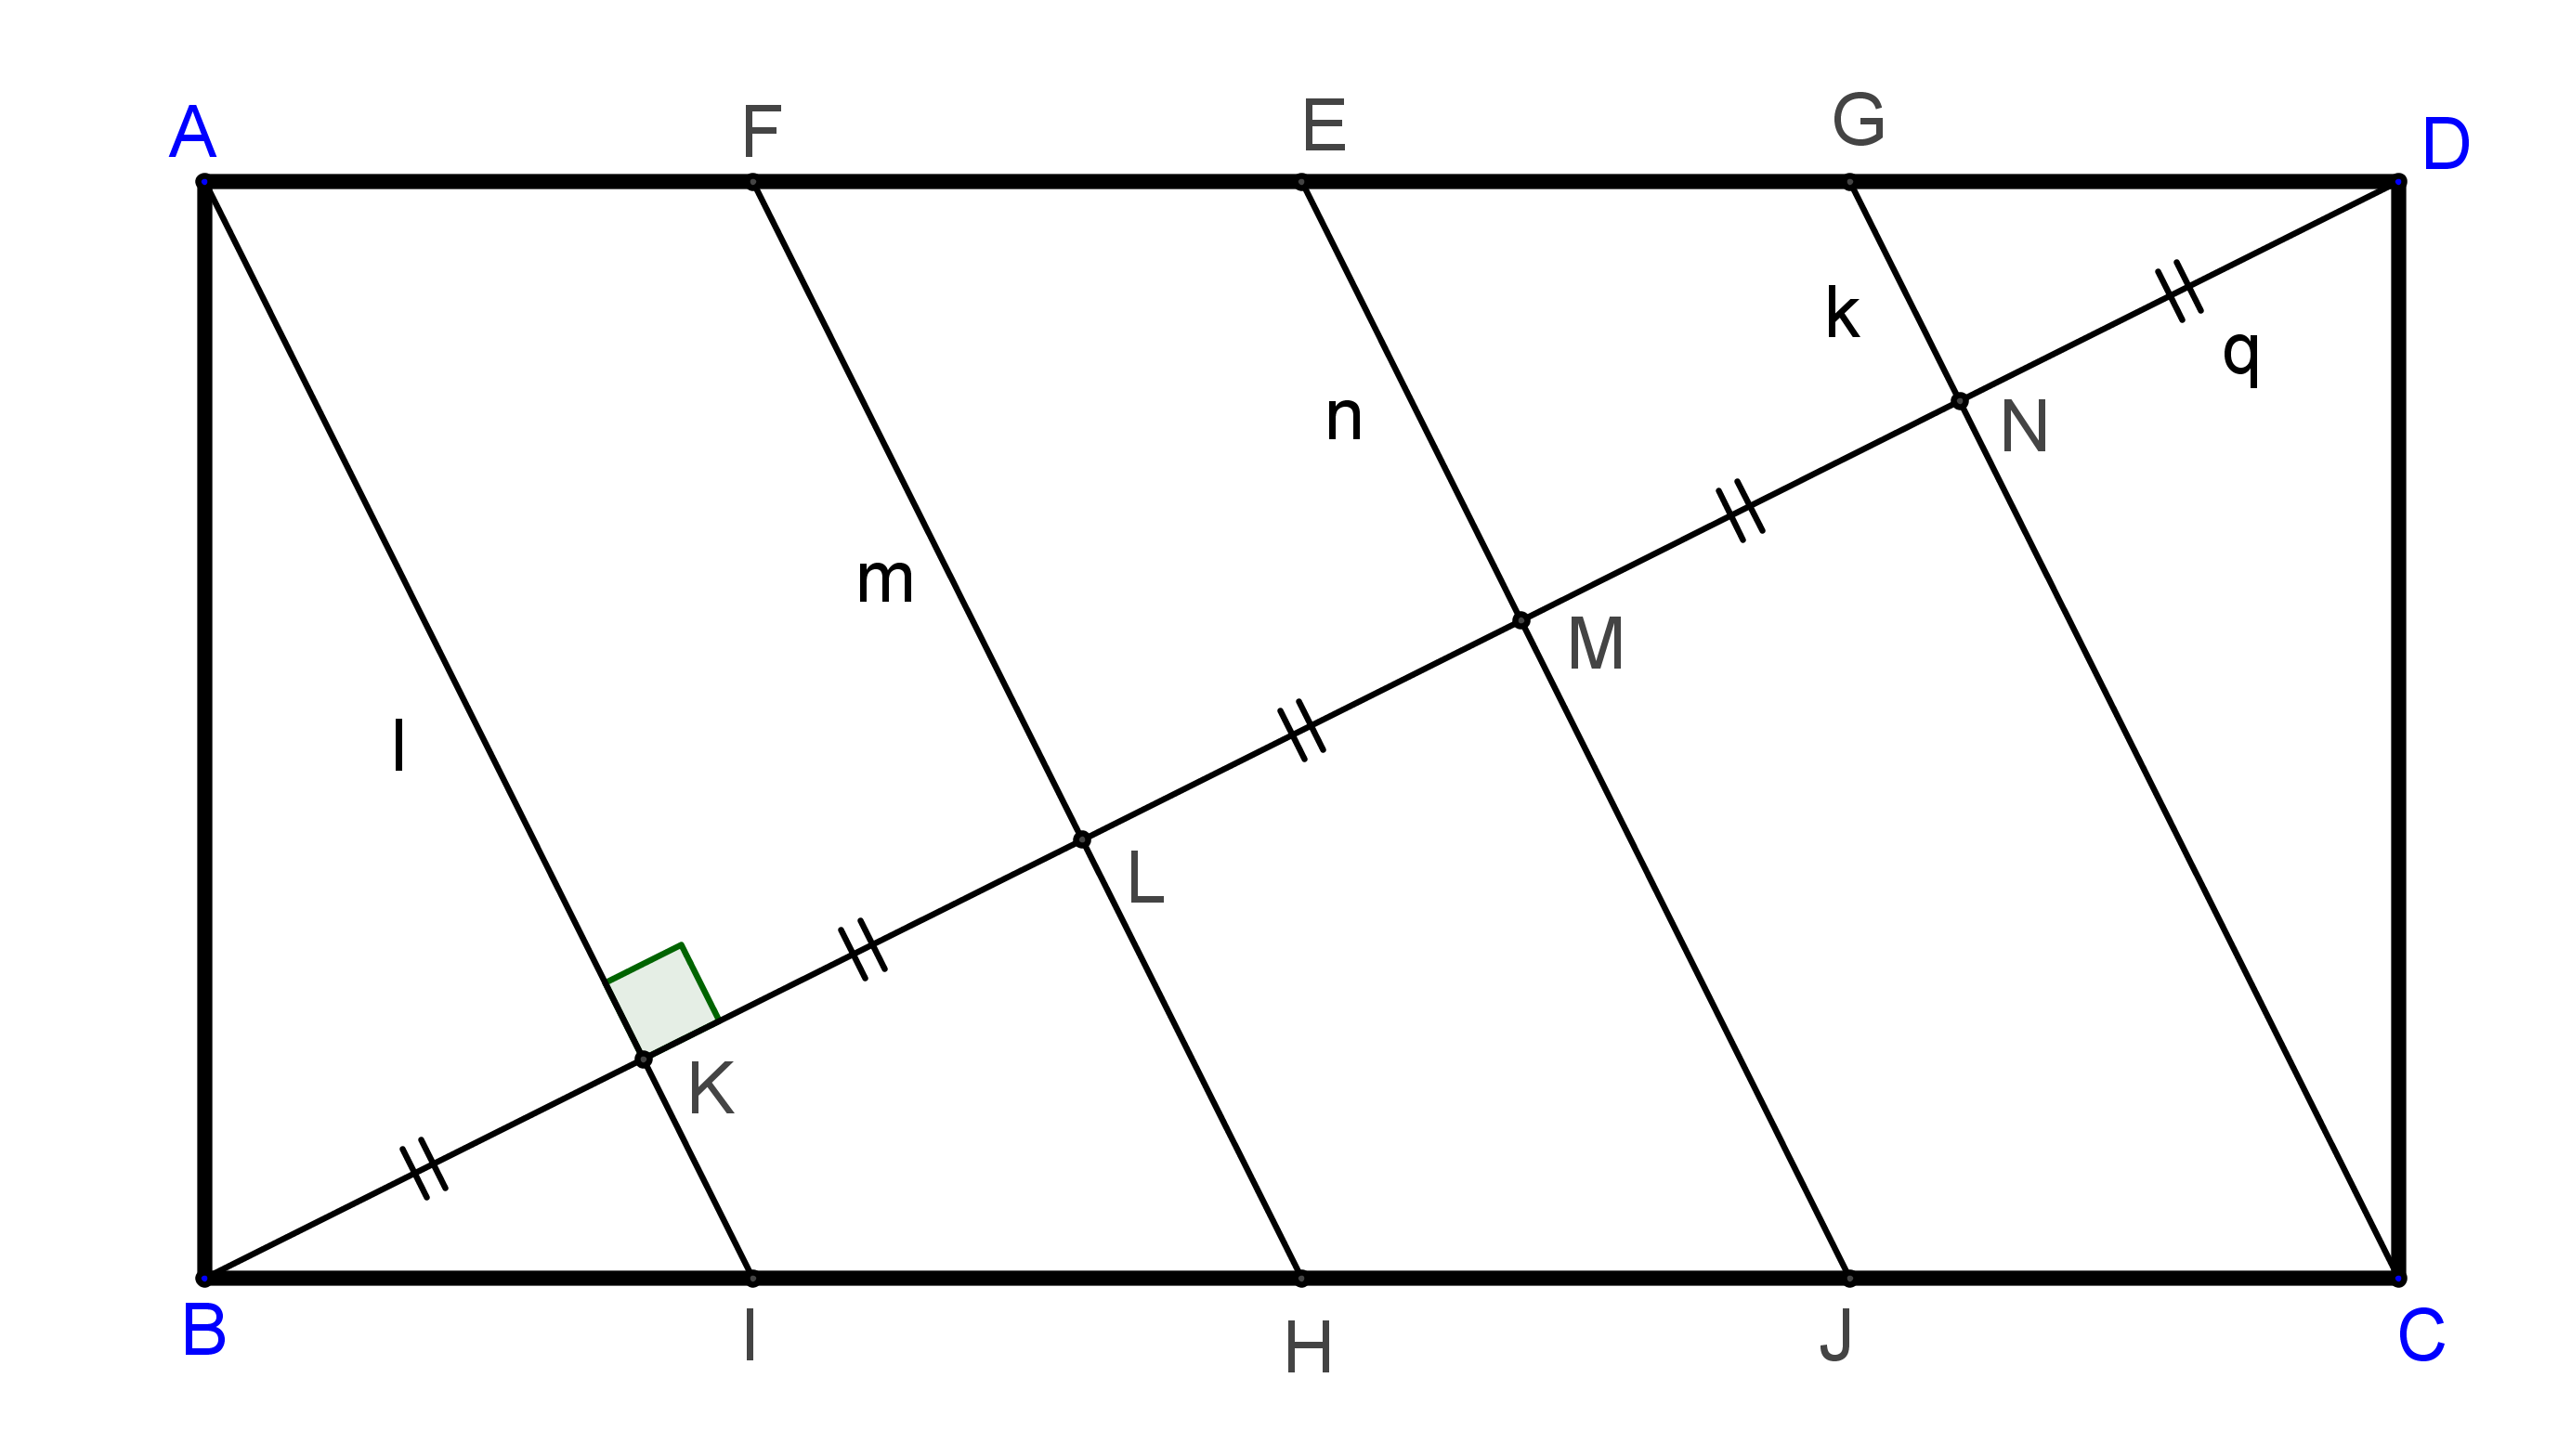
\includegraphics[width=0.5\textwidth]{SSEN_0812}
\ep

\bp{814}
\(\triangle ABC\)와 \(\triangle DCE\)가 서로 닮음이고 \(AB=6\), \(BC=5\), \(CE=10\)일 때 \(DF\)의 길이를 구하여라.
\par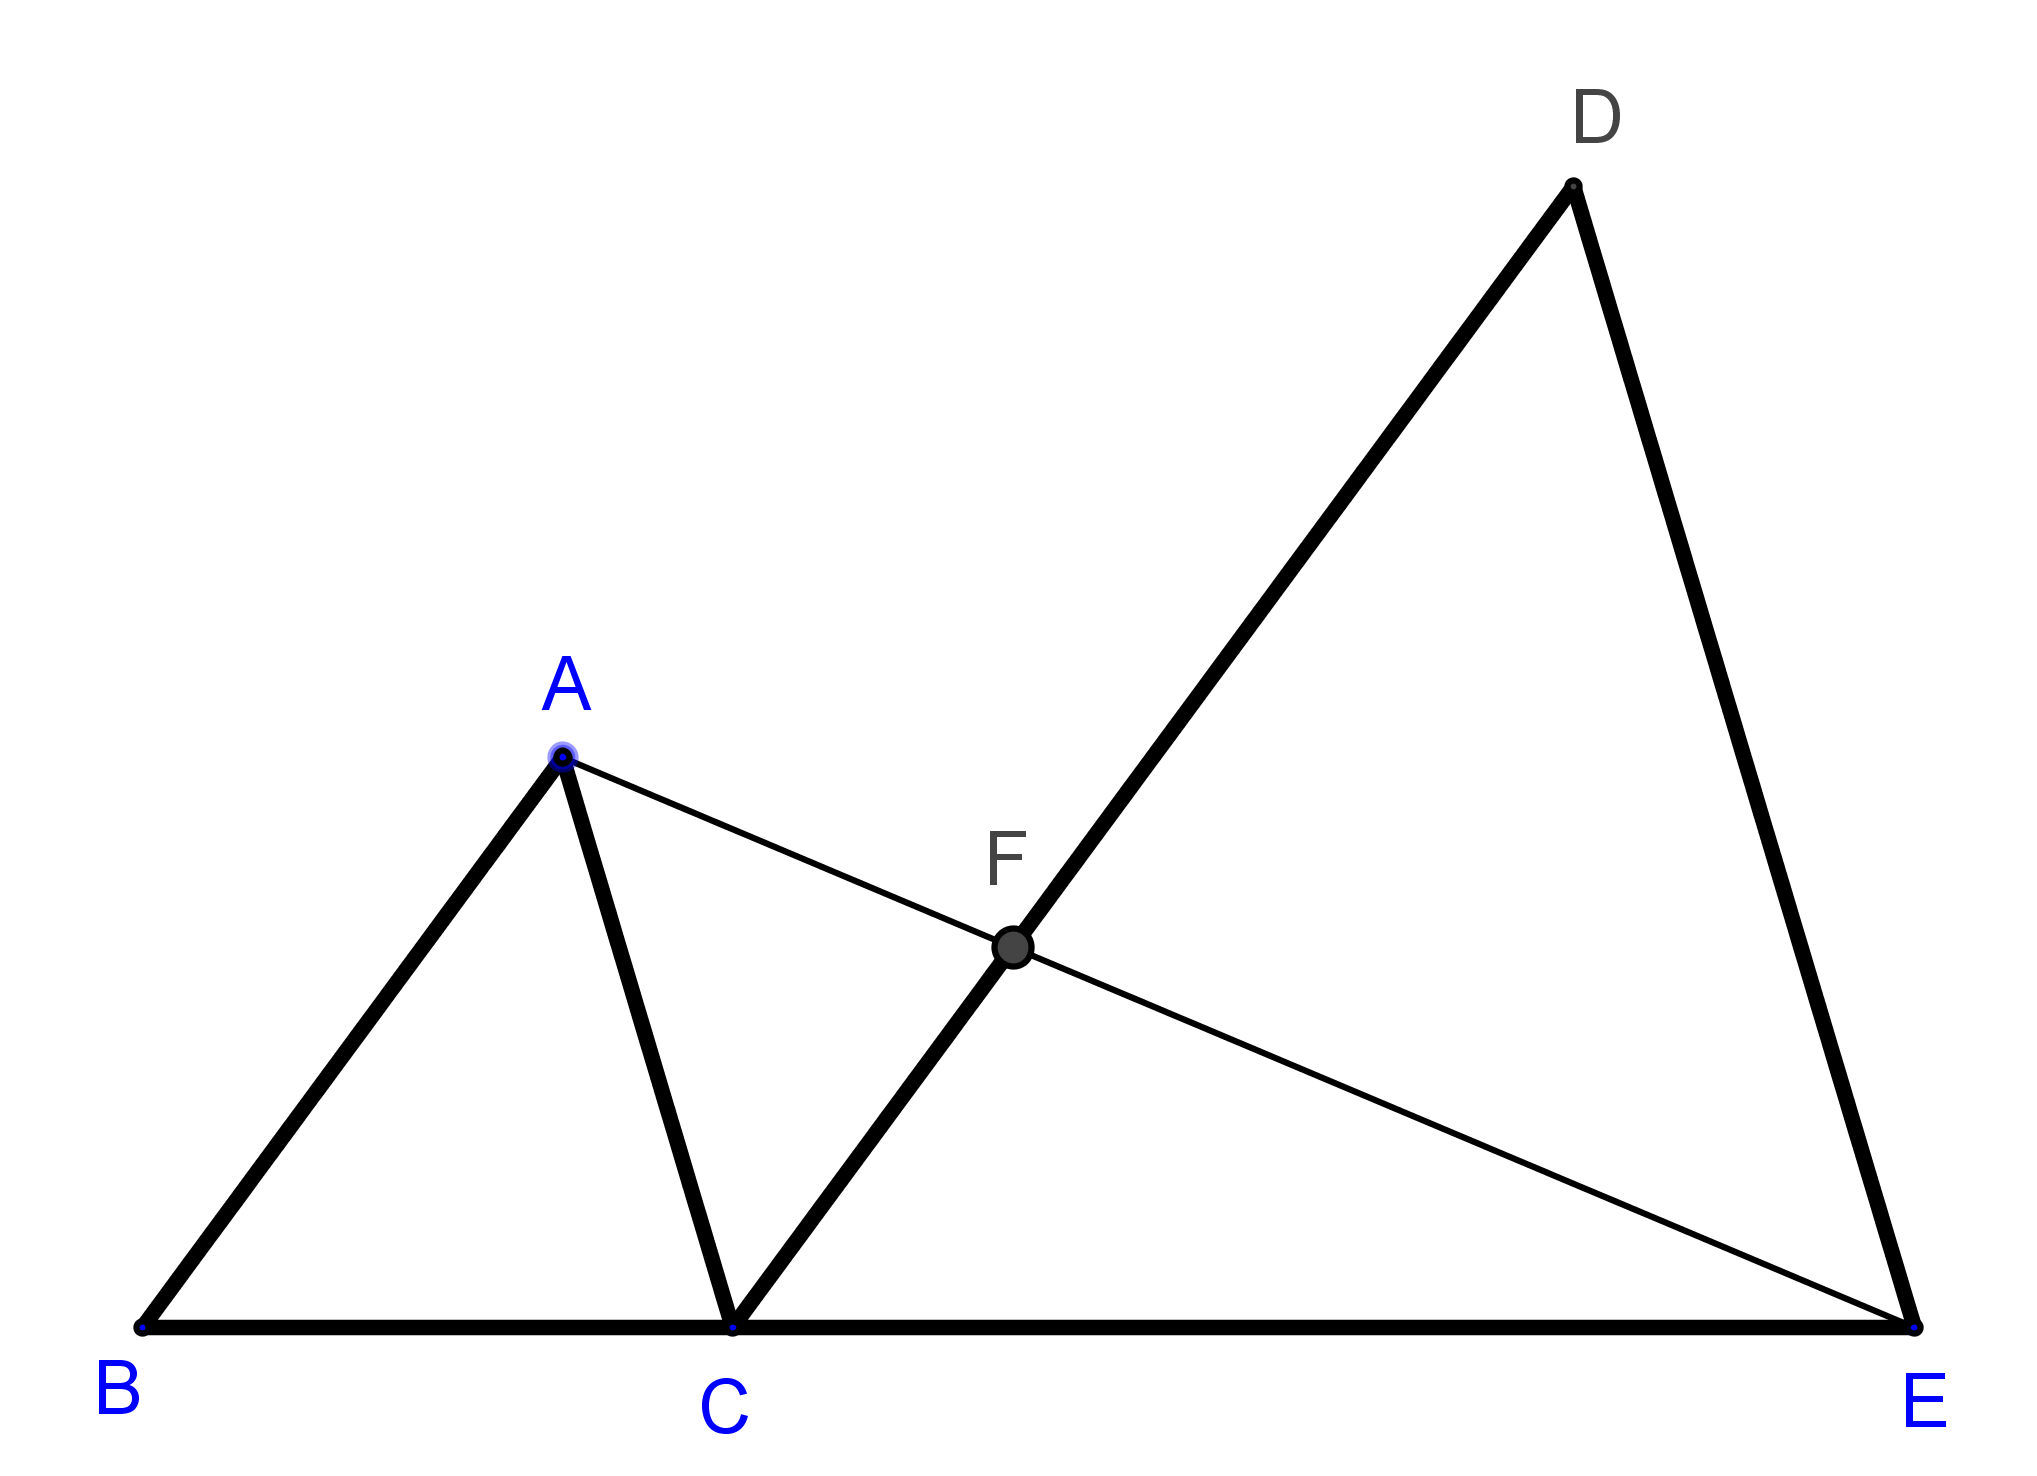
\includegraphics[width=0.5\textwidth]{SSEN_0814}
\ep

\bp{878}
\(\angle BAD=\angle CAD\), \(\angle CAE=\angle FAE\)이고 \(AB=12\), \(BD=3\), \(AC=8\)일 때, \(CE\)의 길이를 구하여라.
\par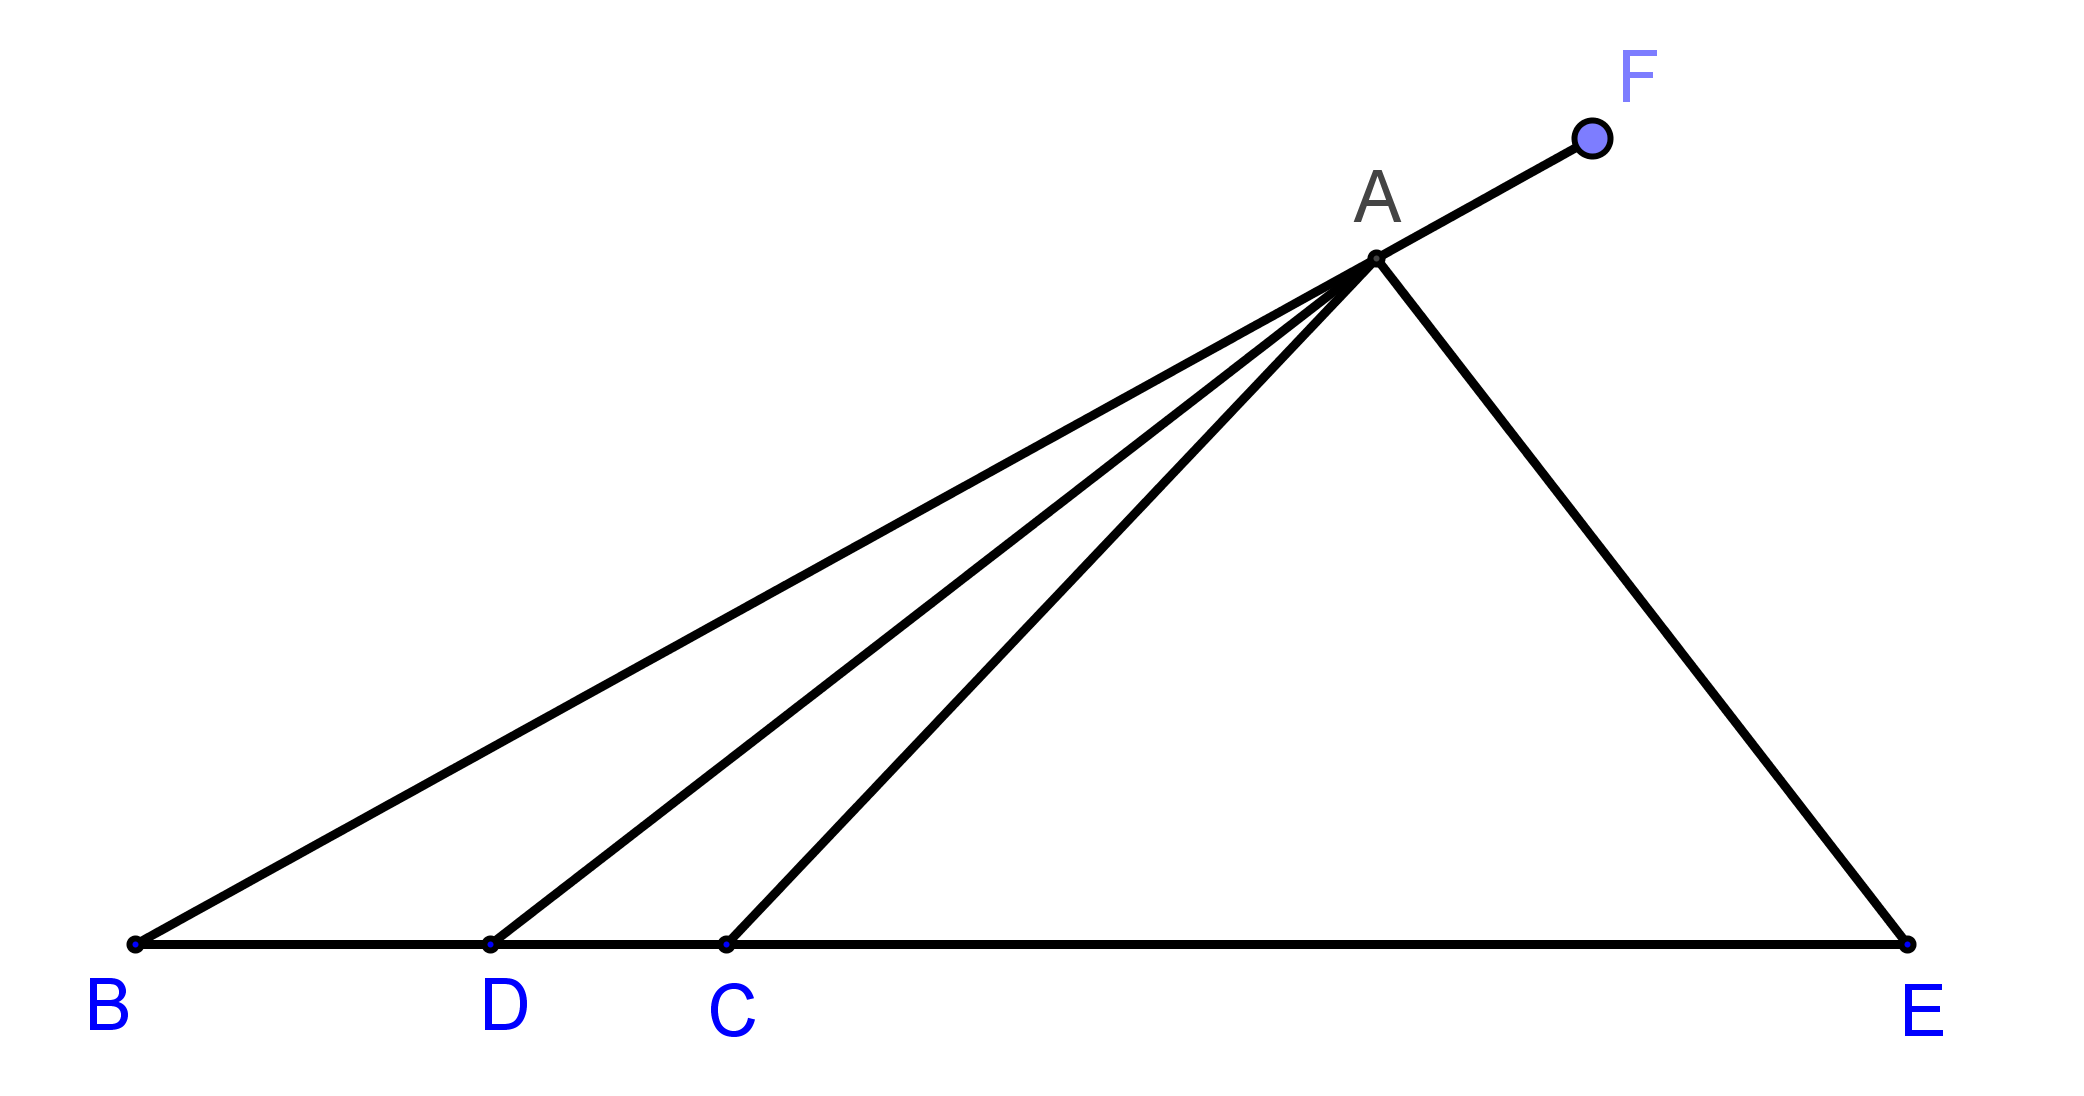
\includegraphics[width=0.7\textwidth]{SSEN_0878}
\ep

\bp{932}
\(AB=8\), \(BC=24\), \(CD=16\)일 때, \(\triangle BCE\)의 넓이를 구하여라.
\par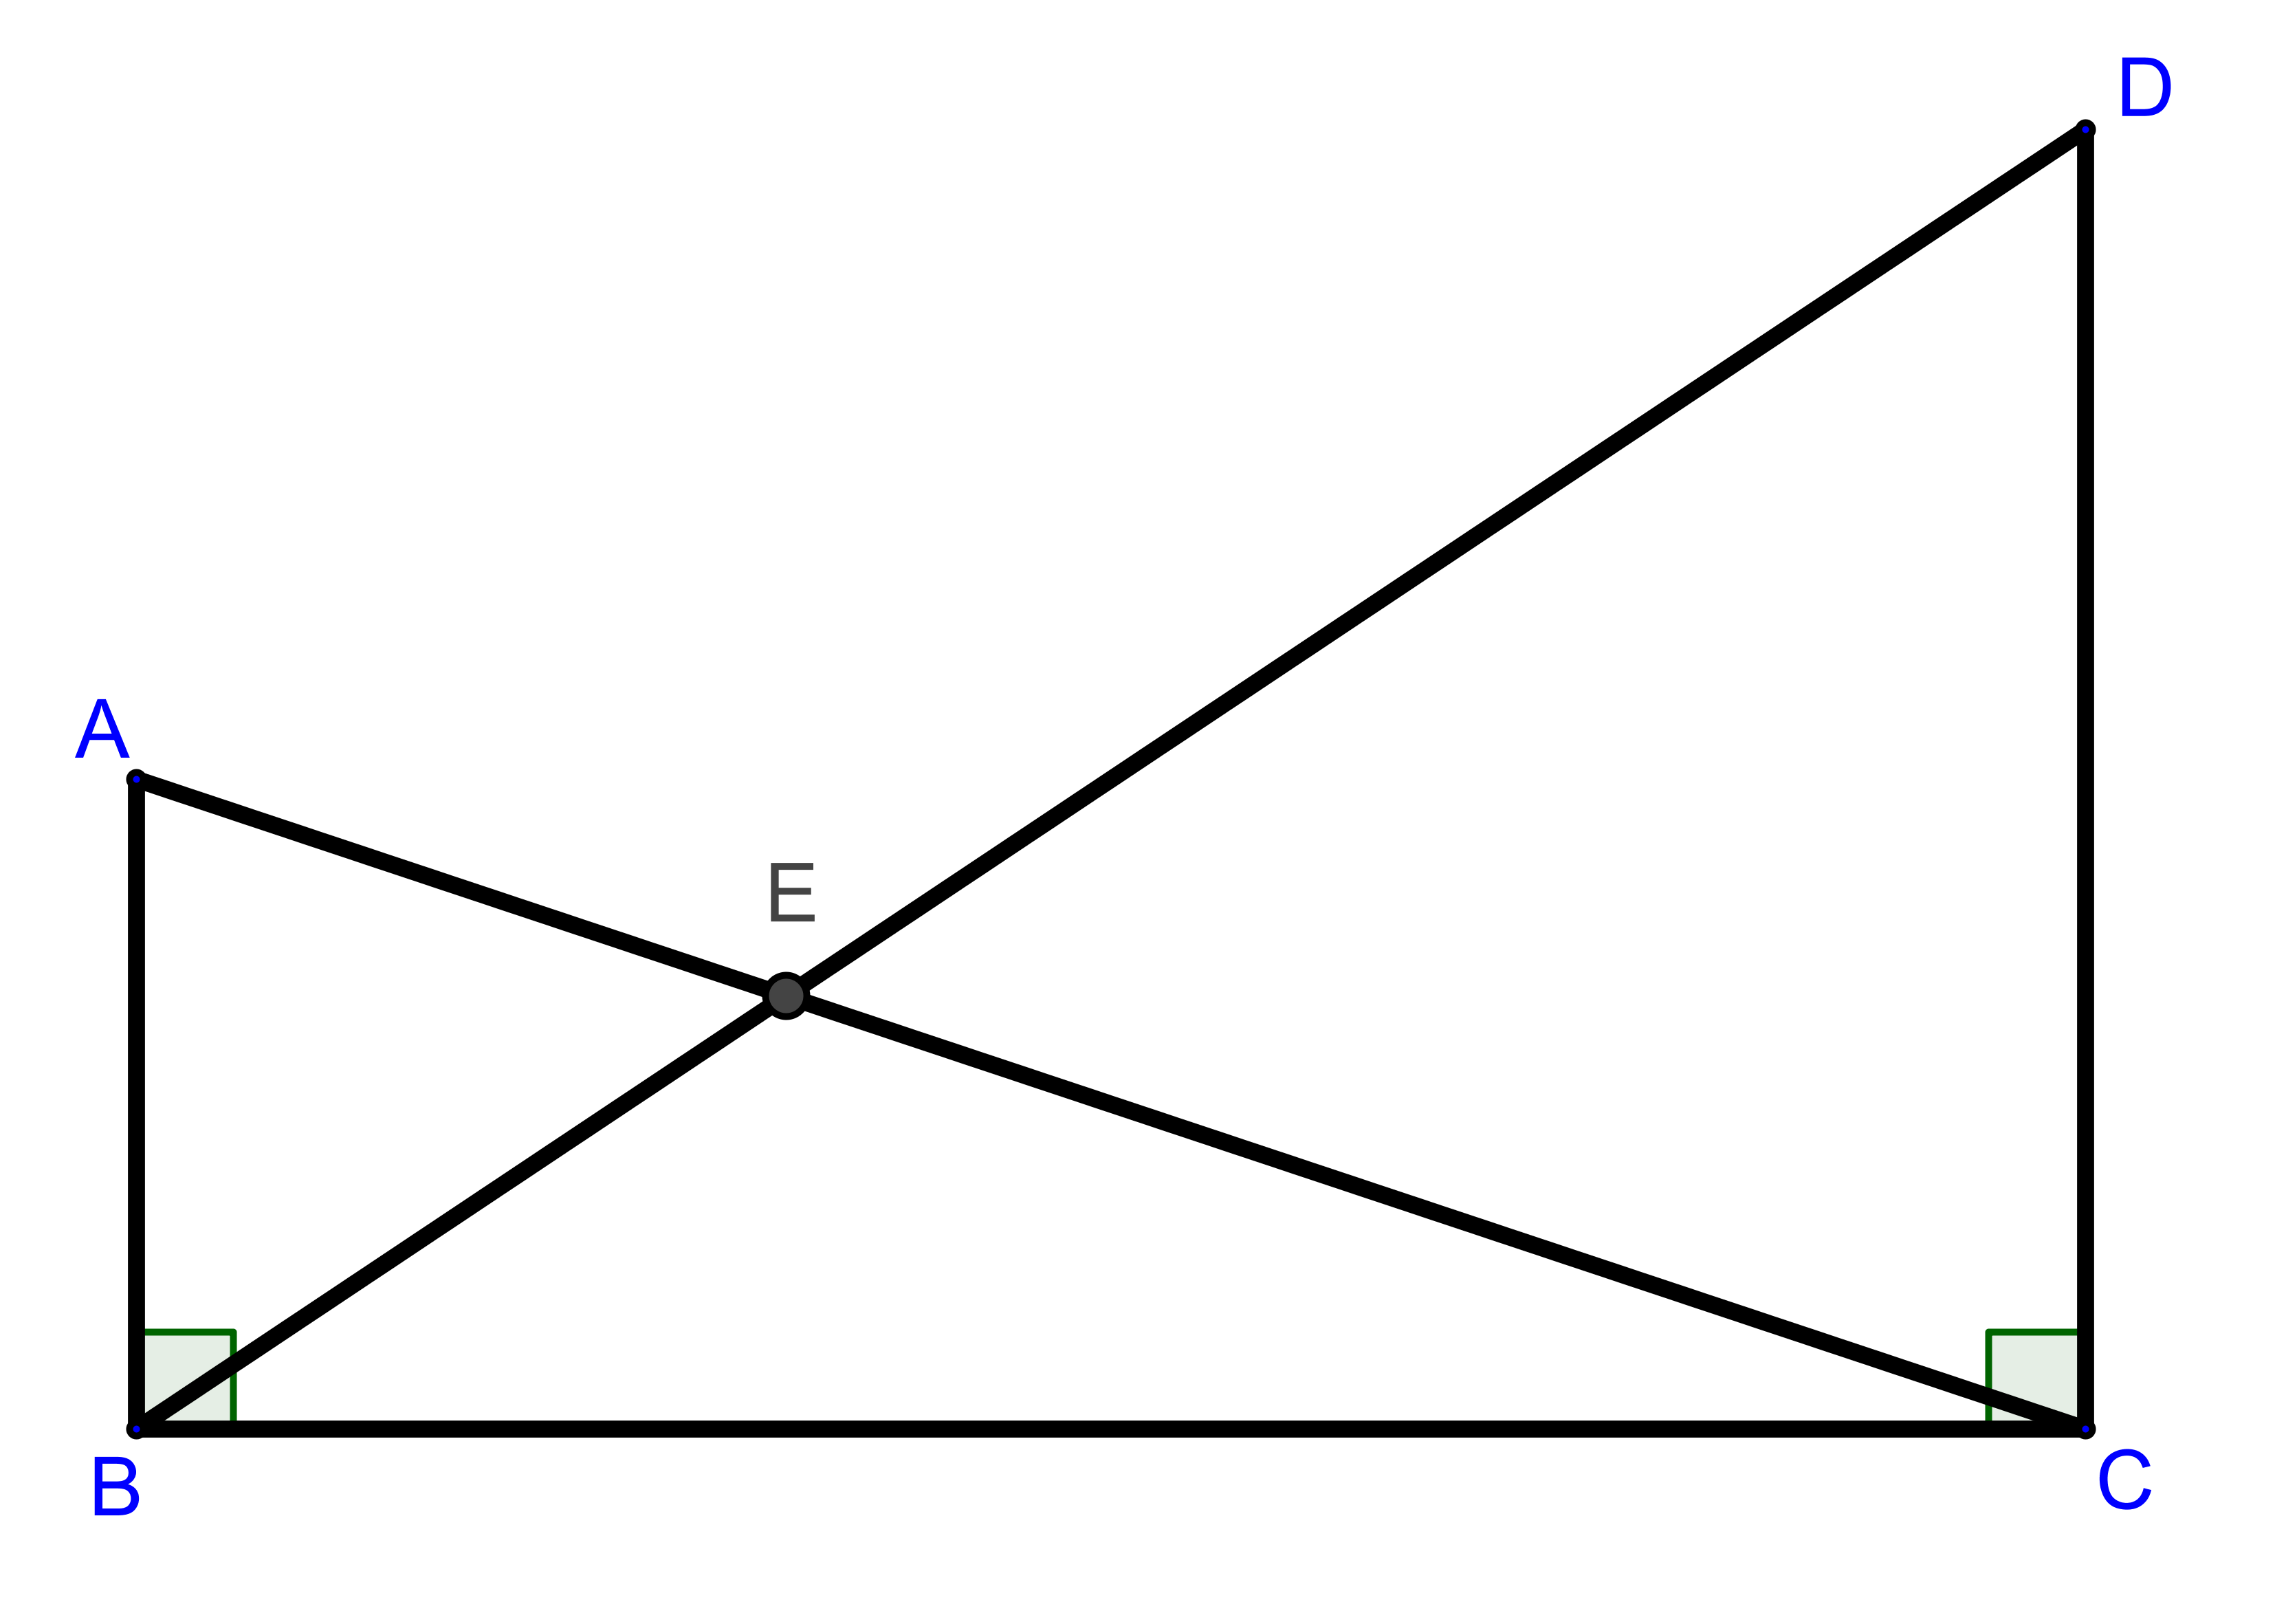
\includegraphics[width=0.5\textwidth]{SSEN_0932}
\ep

\bp{936}
\(AB=5\), \(BC=10\), \(CA=9\)일 때, \(EP\)의 길이를 구하여라.
\par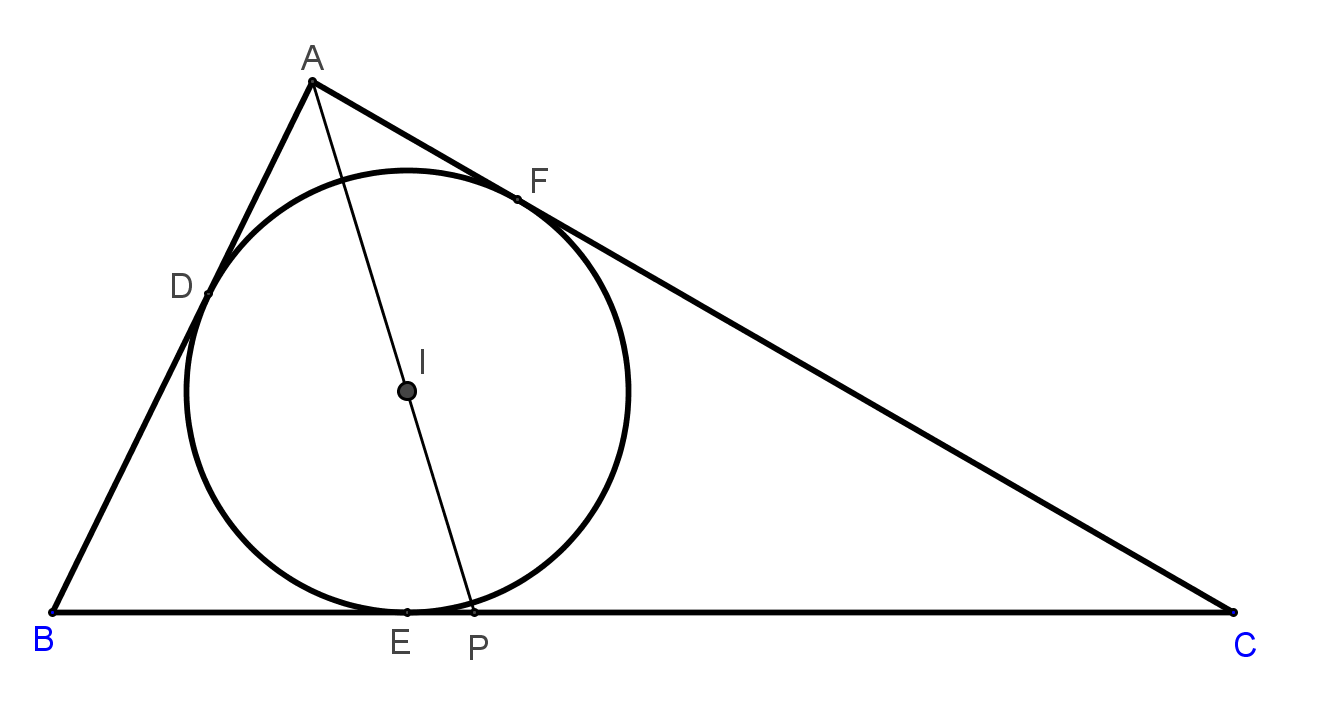
\includegraphics[width=0.5\textwidth]{SSEN_0936}
\ep

\bp{949}
등변사다리꼴 \(ABCD\)에 대해 \(\angle MPQ\)의 크기를 구하여라.
\par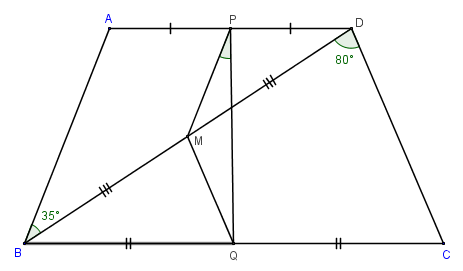
\includegraphics[width=0.5\textwidth]{SSEN_0949}
\ep

\bp{1019}
\(AB=4\), \(AC=3\)일 때 \(\triangle ADE\)의 넓이를 구하여라.
\par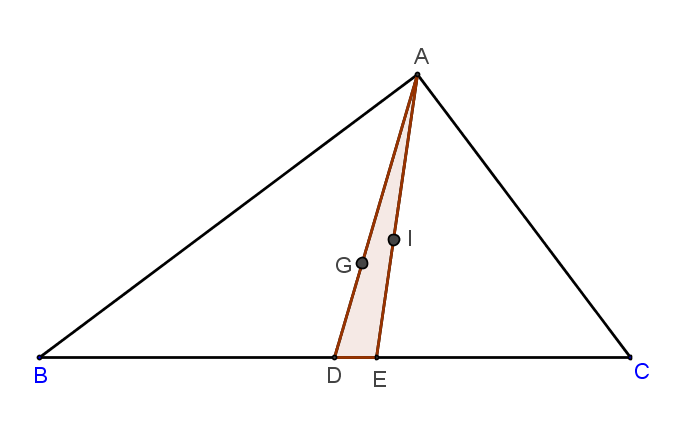
\includegraphics[width=0.5\textwidth]{SSEN_1019}
\ep

\bp{1077}
\(BF:CF=1:2\)이고 \(\triangle ABC=72\)일 때 \(\triangle GBF\)의 넓이를 구하여라.
\par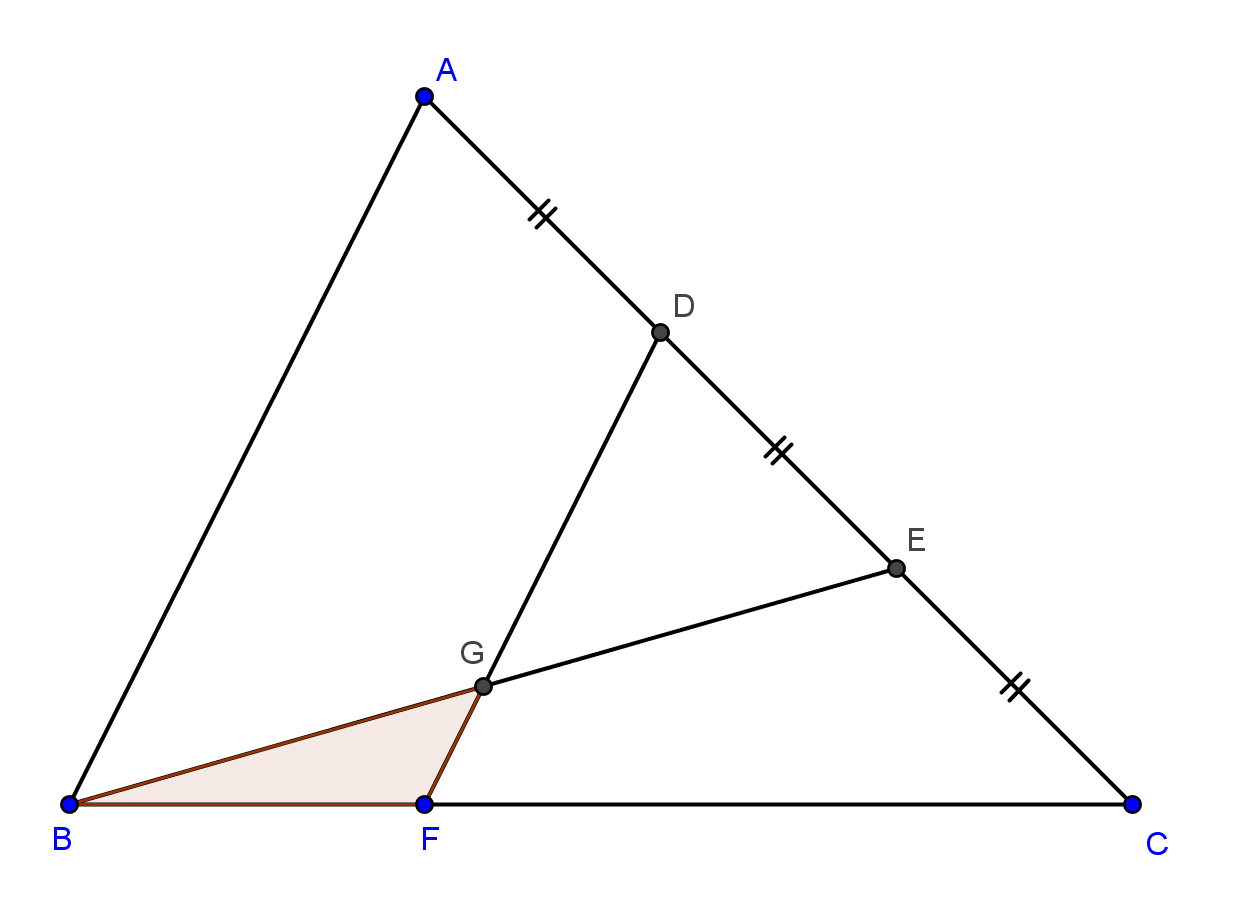
\includegraphics[width=0.5\textwidth]{SSEN_1077}
\ep
\end{document}